\chapter{Preliminaries}

\section{Notation}

\begin{itemize}
\item $2^X$ is the set of~all subsets of a~set~$X$, that is $\{ S \st
S\subseteq X \}$.

\item $A \Subset B$ means that {\sl set $A$ is a finite subset of set $B$\/}.

\item $\overline{S}$ is the~closure of $S$ in a~given topology.
It is defined by
\[
  \overline{S} = \bigcap_{ \text{closed } A\colon \, A\supseteq S} A
  \, ,
\]
or equivalently,
\[
  \overline{S} = \{ x \st U \text{ is open and } U\owns x \Rightarrow U \cap S
  \ne \none \}.
\]

\end{itemize}

\section{Definitions}

\subsection*{Order theory}

\begin{itemize}
\item A~\emph{preorder} is a~binary relation $\sqsubseteq$ that is
  \begin{description}
  \item[(reflexive)] $a \sqsubseteq a$
  \item[(transitive)] $a \sqsubseteq b \text{ and } b \sqsubseteq c \Rightarrow
  a \sqsubseteq c$.
  \end{description}

\item A~\emph{pseudocomplement} of an element $x$ is $x^*$ such that $y \le x^*
\equiv x \wedge y = 0$.
\end{itemize}

\begin{fact}
  $x \le x^{**}$.
  (As the $x$, among others, meets with $x^*$ in $x^* \wedge x = 0$.)
\end{fact}

\begin{itemize}
\item A relation $R$ \emph{interpolates} if $R \subseteq R \circ R$.

\item Monotone maps $l\colon A \to B$ and $r\colon B \to A$ are \emph{Galois
  adjoints\/} ($l$ is a~\emph{left adjoint\/} of $r$ and $r$ is a~\emph{right
  adjoint\/} of $l$) if for every $a\in A, \, b\in B$
  \[
    l(a) \le b \; \equiv \; a \le r(b).
  \]
\end{itemize}

\begin{rem}
  Adjoints are unique:\thinspace%
  \footnote{if they exist}
  $l(a) \le b \; \equiv a \le r(b) \; \equiv \; l'(a) \le b$ leads to
  \begin{align*}
    l(a) \le l'(a) \; &\equiv \; l'(a) \le l'(a) \\
    \text{and } l(a) \le l(a) \; &\equiv \; l'(a) \le l(a)
  \end{align*}
  and hence $l(a) = l'(a)$ for $a\in A$.
  Symmetrically for right adjoints.
\end{rem}

\begin{fact} \label{lr-id-rl}
  $lr \le id$ resp. $id \le rl$.
  (Set $a := r(b)$ resp. $b := l(a)$.)
\end{fact}

\begin{fact} \label{lrl=l}
  $lrl = l$.
  (Following from Fact~\ref{lr-id-rl} and the monotonicity of $l$ we get $l \le
   lrl$.
  On~the~other hand, $lr(b) \le b$ with $b := l(a)$ gives us $lrl \le l$.)
\end{fact}

\begin{itemize}
\item $f^*$ resp. $f_*$ is the~left resp. right adjoint of $f$.

\item $\left\downarrow U \right. = \bigcup_{u\in U} \{x \st x \le u\}$ and
$\left\uparrow U \right. = \bigcup_{u\in U} \{x \st x \ge u\}$.
Especially,
\[
  \left\downarrow a \right. = \{x \st x \le a\} \text{ and } \left\uparrow a
  \right. = \{x \st x \ge a\}.
\]

\item A~set $U$ is a~\emph{down-set\/} resp. an~\emph{up-set\/} if
$\left\downarrow U \right. = U$ resp. $\left\uparrow U \right. = U$.

\item Let $X$ be a~partially ordered set.
Then $\D(X)$ is the set of~all down-sets in~$X$ ordered by inclusion.

\item We say that $p \ne 1$ is \emph{prime\/} when
\[
  x_1 \wedge x_2 \le p \; \Longrightarrow x_1 \;
  \le p \text{ or } x_2 \le p,
\]
and \emph{semiprime\/} when
\[
  x_1 \wedge x_2 = 0 \; \Longrightarrow \;
  x_1 \le p \text{ or } x_2 \le p.
\]
\end{itemize}

\begin{lem} \label{lem:primeness-equiv}
  In a~distributive lattice an~element~$p \ne 1$ is prime iff 
  \[
    x_1 \wedge x_2 = p \; \Longrightarrow \; x_1 = p \text{ or } x_2 = p.
  \]
\end{lem}
\begin{proof}
  $\Rightarrow$:
  If $x_1 \wedge x_2 = p$ then there is $x_i \le p$ by primeness and since $x_j
  \ge x_1 \wedge x_2$ for $j\in \{ 1, 2 \}$ then also $x_i \ge p$.

  $\Leftarrow$:
  We have $(x_1 \vee p) \wedge (x_2 \vee p) = (x_1 \wedge x_2) \vee p = p$.
  Hence, for some $i\in \{ 1, 2 \}$ we get $x_i \vee p = p$, that is, $x_i \le
  p$.
\end{proof}

\begin{itemize}
\item An~\emph{atom\/} resp. a~\emph{coatom\/} is an~element $a > 0$ resp. $a <
1$ such that
\begin{align*}
  0 < x \le a &\Rightarrow x = a ~~~~~~\\
  \text{resp. } a \le x < 1 &\Rightarrow x = a.
\end{align*}

\item For $a < b$ we say that \emph{$a$ is covered by $b$\/} and write $a \cov
b$ if
\[
  a < x \le b \Rightarrow x = b.
\]

\item An element $a$ is said to be \emph{covered\/} if it is covered by some
$b$.

\end{itemize}

\subsection*{Category theory}

\begin{itemize}
\item A \emph{category} $\Ccal$ is a collection consisting of
  \begin{itemize}
  \item class~$ob(\Ccal)$ of \emph{objects\/}
  \item class~$morph(\Ccal)$ of \emph{morphisms\/} between objects\thinspace%
  \footnote{a~morphism $f$ between objects $A$ and $B$ is indicated by $f\colon
    A \to B$}
  \end{itemize}
further satisfying the axioms of
  \begin{itemize}
  \item \emph{(identity)\/}
  For every $X\in ob(\Ccal)$ there is a~morphism $1_X$ such that for any
  $f\colon A \to B$ we have $1_B \cdot f = f = f \cdot 1_A$.
  \item \emph{(asociativity)\/}
  Whenever $f\colon A \to B$, $g\colon B \to C$ and $h\colon C \to D$ then also $h
  \cdot (g \cdot f) = (h \cdot g) \cdot f$.
  \end{itemize}

\item The \emph{opposite category}~$\mathcal{C}^{op}$ of a category
$\mathcal{C}$ has the same objects $ob(\Ccal)$ and reverses the composition.
Thus a~morphism $A \to B$ goes now from $B$ to $A$.

\item Let objects of a~category $\Ccal$ be structured sets, their morphisms be
maps (respecting the structure in that or other way) and the composition
of~morphisms be same as the composition of~maps.
Then $\Ccal$ is called \emph{concrete\/}.

\item An~\emph{epimorphism} is a~right-cancellative morphism $e$, that is,
\[
  f_1 \cdot e = f_2 \cdot e \; \Longrightarrow \; f_1 = f_2.
\]

\item A~\emph{monomorphism} is a~left-cancellative morphism $m$:
\[
  m \cdot f_1 = m \cdot f_2 \; \Longrightarrow \; f_1 = f_2.
\]

We also refer to these by saying that \emph{$e$ is epic\/} and \emph{$m$ is
monic\/}.
\end{itemize}

\begin{fact} \label{fct:onto->epic}
  In a~concrete category every morphism onto resp. one-one is epic resp. monic.
\end{fact}
(Else there would be $x$ with $f_1(x) \ne f_2(x)$.
 From surjectivity, the existence of~$z$ such that $e(z) = x$ would lead to
 $f_1 \cdot e(z) \ne f_2 \cdot e(z)$;
 and if $m$ is one-one then $m \cdot f_1(x) \ne m \cdot f_2(x)$.
 )

\begin{itemize}
\item An \emph{isomorphism} is a~morphism $f\colon A \to B$ that has
an~\emph{inverse morphism\/} $\overline{f}\colon B \to A$ such that
\[
  \overline{f} \cdot f = 1_A \text{ and } f \cdot \overline{f} = 1_B.
\]
\end{itemize}

\begin{itemize}
\item A \emph{product} of a system $\left(A_i\right)_{i\in J}$ is a~system
of~\emph{projections\/}
\[
  \left(p_i\colon \prod_{j\in J} A_j \to A_i \right)_{i\in J}
\]
with the property that for an~arbitrary system $\left(f_i\colon X \to
A_i\right)_{i\in J}$ there is a~unique solution~$f\colon X \to \prod_{j\in
J} A_j$ to equations
\[
  p_i \cdot f = f_i \text{ for } i\in J.
\]

\item Similarly, a \emph{coproduct} is a~system of~\emph{injections\/}
\[
  \left(\iota_i\colon A_i \to \coprod_{j\in J} A_j \right)_{i\in J}
\]
such that any $\left(g_i\colon A_i \to X \right)_{i\in J}$ has a~single
solution~$g\colon \coprod_{j\in J} A_j \to X$ to~equations
\[
  g \cdot \iota_i = g_i \text{ for } i\in J.
\]
Note that this is a~product in the~opposite category.

\item The~\emph{diagonal} is the (only) morphism $\Delta\colon A \to \prod_{i\in
J} A$ solving the system $p_i\cdot \Delta = 1_A$ for $i \in J$.
Dually, the~\emph{codiagonal} is the solution $\nabla\colon \coprod_{i\in J} A
\to A$ to the system $\nabla\cdot \iota_i = 1_A$ for $i \in J$.
\end{itemize}


\subsection*{Point-set topology}

\begin{itemize}
\item A \emph{topology} on a~set~$X$ is a~system~$\tau\subseteq 2^X$ satisfying
the axioms
  \begin{description}
  \item[(o1)] $\none, X \in \tau$
  \item[(o2)] $\left\{ U_i \st i\in J \right\} \subseteq \tau \; \Rightarrow \;
  \bigcup_{i\in J} U_i \in \tau$
  \item[(o3)] $U_1, U_2 \in \tau \; \Rightarrow \; U_1 \cap U_2 \in \tau$.
  \end{description}

\item The $U\in \tau$ are referred to as \emph{open sets\/} and $(X, \tau)$ as
a~\emph{topological space\/}.

\item We often abbreviate $(X, \tau)$ to $X$;
then $\tau$ is usually indicated by~$\Omega(X)$.

\item The complements of open sets are referred to as \emph{closed sets\/}.

\item A~\emph{basis} of a~topology~$\tau$ is $\mathcal{B}\subseteq \tau$ such
that for every open $U$ we can write $U = \bigcup \{V\in \mathcal{B} \st
V\subseteq U \}$.

\item $\mathcal{S}\subseteq \tau$ is a~\emph{subbasis} of a~topology~$\tau$ if
$\left\{ \bigcap \mathcal{F} \st \mathcal{F} \Subset \mathcal{S} \right\}$ is
a~basis of~$\tau$.
\end{itemize}

\begin{exmpl}
  $\{ \langle 0, a \langle, \; \rangle a, 1 \rangle \st 0
  < a < 1 \}$ is a~subbasis of~the standard topology of~the interval $\langle
  0, 1\rangle$.
\end{exmpl}

\begin{itemize}
\item A~function~$f\colon X \to Y$ between topological spaces $X$ and $Y$ is
\emph{continuous} if 
\[
  U\in \Omega(Y) \; \Longrightarrow \; f^{-1}[U]\in \Omega(X).
\]
Since the preimage function preserves unions and finite intersections, it
suffices to require that $f^{-1}[U]$ be open for all \emph{subbasic\/} $U$.
\end{itemize}

\begin{exmpl}
  The topological space $\left( \prod_{i\in J} X_i, \mathcal{S} \right)$ with
  the subbasis
  \[
    \mathcal{S} = \left\{ p_{i}^{-1}[U] \st i\in J, \; U\in \tau_i \right\}
  \]
  is the product of topological spaces $\left( X_i \right)_{i\in J}$;
  more precisely, the projections
  \[
    \left( p_i\colon \left(\prod_{i\in J} X_i, \mathcal{S}\right) \to
    \left(X_i, \tau_i\right) \right)_{i\in J}
  \]
  constitute the product in~the~category~{\bf Top} (of~topological spaces and
  continuous functions).
\end{exmpl}

\subsection*{Point-free topology}

\begin{itemize}
\item A~\emph{frame} is a~complete lattice $L$ satisfying the distributivity
law
\[
  b \wedge \bigvee A = \bigvee \{ b \wedge a \st a\in A \}
\]
for every $A\subseteq L$ and $b\in L$.

\item For a~topological space $X$ the set~$\Omega(X)$ ordered by~inclusion is
a~frame:
by~axioms {\bf (o2)} and {\bf (o3)} (see ``Point-set topology'') operations
$\wedge$ resp. $\bigvee$ coincide with $\cap$ resp. $\bigcup$.

\item A \emph{frame homomorphism} between frames $M$ and $L$ is a~map $h\colon
M \to L$ preserving all joins (in particular, $h(0) = 0$) and~all finite meets
(especially, $h(1) = 1$).

\item The category of~frames and frame homomorphisms will be denoted by {\bf
Frm}.

\item The objects of the~opposite category~{\bf Loc} are called
\emph{locales\/}.
The morphisms of {\bf Loc} can be represented as follows:

  \begin{itemize}
  \item A \emph{localic map} between locales $L$ and $M$ is a mapping $f\colon L
  \to M$ with left Galois adjoints $f^*\colon M \to L$ such that $f^*$ is a frame
  homomorphism.
  Thus, localic maps are infima-preserving maps such that their left adjoints
  preserve finite meets.
  \end{itemize}

\item A \emph{sublocale} of locale $L$ is a $S\subseteq L$ satisfying
  \begin{description}
  \item[(S1)] $M\subseteq S \Longrightarrow \bigwedge M\in S$
  \item[(S2)] $x\in L \text{ and } s\in S \Longrightarrow x \rightarrow s \in S$.
  \end{description}
\end{itemize}

\begin{fact}
  The set-theoretic image $f[L]$ under a localic map $f\colon L\to M$
  is a~sublocale of~$M$.
\end{fact}

\begin{itemize}
\item Each $\left\uparrow a\right.$ is a~sublocale.
These sublocales are referred to as \emph{closed sublocales\/}.
\end{itemize}

\begin{rem}[Sublocale homomorphisms]
  There is an~alternative representation of~sublocales:
  \begin{itemize}
    \item A~\emph{sublocale\/} of a~locale~$L$ is a~frame homomorphism $h\colon
    L \to M$ that is onto.
    For sublocales $h\colon L \to M$, $h'\colon L \to M'$ we have the preorder:
    \[
      h \sqsubseteq h'
    \]
    if there is a~frame homomorphism $\alpha\colon M' \to M$ such that $\alpha
    h' = h$.

    \item Thus, $h$~and~$h'$ represent the same sublocale iff this $\alpha$ is
    also an~isomorphism.

    \item
    \phantomsection
    \label{df:closed-sloc}
    In this representation \emph{closed sublocales\/} are frame homomorphisms
    which are of~the form
    \[
      \check{a} = (x \mapsto a \vee x) \colon L \to \left\uparrow a \right.
    \]
    for $a\in L$.
  \end{itemize}
\end{rem}

\begin{lem} \label{lem:embed-adjoint}
  The embedding $j = (x \mapsto x)\colon \left\uparrow a \right. \embed L$ is
  the right adjoint to~$\check{a}$.
\end{lem}
\begin{proof}
  For $x\in L$ and $y\in \left\uparrow a \right.$ we will show that $x \vee a =
  \check{a}(x) \le y$ iff $x \le j(y) = y$.

  $\Rightarrow$:
  Immediately from $x \le x \vee a$.

  $\Leftarrow$:
  Following from $y \ge x$ and $y \ge a$.
\end{proof}

\begin{itemize}
  \item The \emph{closure\/} of~a~sublocale $h\colon L \to M$ is the
  $\sqsubseteq$-least closed sublocale~$f$ such that $f \sqsupseteq h$.
\end{itemize}

\begin{prop} \label{prop:sloc-closure}
  For a~locale $L$ and any of~its sublocales $h\colon L \to M$ let
  \[
    c := \bigvee \{ x \st h(x) = 0 \}.
  \]
  Then $\check{c}\colon L \to \left\uparrow c \right.$ is the closure of~$h$.
\end{prop}
\begin{proof}
  Firstly, $\check{c} \sqsupseteq h$:
  we will find $\gamma\colon \left\uparrow c \right. \to M$ with $\gamma
  \check{c} = h$.
  For every $y\in \left\uparrow c \right.$ take $x\in L$ such that $y =
  x \vee c$ and set $\gamma(y) := h(x)$.
  It is a~correct definition:
  since $h(c) = \bigvee \{ h(x) \st h(x) = 0 \} = 0$,
  if $x_1 \vee c = x_2 \vee c$ then
  \[
    h(x_1)
    = h(x_1) \vee 0
    = h(x_1 \vee c)
    = h(x_2 \vee c)
    = h(x_2) \vee 0
    = h(x_2).
  \]
  Furthermore, $\gamma$ is a~frame homomorphism as $\check{c}$ and $\gamma
  \check{c} = h$ are homomorphisms and $\check{c}$ is onto.
  
  Now suppose $\check{a} \sqsupseteq h$ for some $a\in L$.
  That is, there exists a~frame homomorphism $\alpha\colon \left\uparrow
  a\right. \to M$ with $\alpha\check{a} = h$.
  We have
  \[
    0
    = h(0)
    = \alpha\check{a}(0)
    = \alpha(a \vee 0)
    = \alpha(a \vee a)
    = \alpha\check{a}(a)
    = h(a).
  \]
  From the~definition of~$c$ we see that $a \le c$.
  Set $\psi := (x \mapsto c \vee x)\colon \left\uparrow a\right. \to
  \left\uparrow c\right.$.
  We have $\psi\check{a}(x) = c \vee a \vee x = c \vee x = \check{c}(x)$, and
  consequently, $\check{a} \sqsupseteq \check{c}$.
\end{proof}

With the same notation as above, we get
\begin{cor} \label{cor:closed-sloc}
  A sublocale~$h$ is closed iff there exists a~map $\phi\colon M \to
  \left\uparrow c \right.$ with $\phi h = \check{c}$.
\end{cor}
\begin{proof}
  Since $h$ and $\phi h = \check{c}$ are frame homomorphisms and $h$ is onto,
  $\phi$ is also a~homomorphism.
  Moreover, both $h$ and $\check{c}$ are onto and hence epic, and thus,
  \begin{align*}
    h
    = \gamma \check{c}
    = \gamma \phi h
    &\Longrightarrow
    \gamma \phi = id, \\
    \check{c}
    = \phi h
    = \phi \gamma \check{c}
    &\Longrightarrow
    \phi \gamma = id.
  \end{align*}
  Therefore, $\phi$ and $\gamma$ are mutually inverse isomorphisms.
\end{proof}

\subsubsection*{On coproducts in Frm}

In the category of~frames we have a~coproduct
\[
  \iota_i: L_i \to L_1 \oplus L_2, \, i = 1, 2
\]
(there is a general coproduct but we will need a coproduct of two objects
 only).
It can be constructed as follows.

\begin{itemize}
\item
\phantomsection \label{df:satur}
A down-set $U\subseteq L_1 \times L_2$ is said to be \emph{saturated\/} if for
all systems $(x_i)_{i\in J}$ in $L_1$ resp. $L_2$ and all $y$ in $L_2$ resp.
$L_1$ we have
\begin{align*}
    \{ (x_i, y) \st i\in J \} \subseteq U \, &\Rightarrow \, (\bigvee x_i,
        y)\in U \\
    \text{and } \{ (y, x_i) \st i\in J \} \subseteq U \, &\Rightarrow \, (y,
        \bigvee x_i)\in U.
  \end{align*}

\item The definition above concerns also the void $J$ and hence for each
saturated down-set~$U$ we get
\[
  U\supseteq \n := \{ (x, y) \st x = 0 \text{ or } y = 0 \}.
\]
Since $\n$ itself is obviously saturated, it is \emph{the least saturated
down-set\/}.

\item $L_1 \oplus L_2$ will be the set of~all saturated elements in $\D(L_1
\times L_2)$.
In other words, $L_1 \oplus L_2$ is the frame of~all saturated down-sets of
$L_1 \times L_2$ ordered by~the~inclusion.
\end{itemize}

\begin{prop}
For $(a, b)\in L_1 \times L_2$ the down-set
\[
  \darr (a, b) \cup \n
\]
is saturated.
\end{prop}
\begin{proof}
  Let $(x_i, y)\in \darr (a, b) \cup \n$ for $i\in J$.

  \underline{Case $y = 0$}:
  evidently, $(\bigvee_{i\in J} x_i, y) \in \n$.

  \underline{Case $y \ne 0$ and $\bigvee x_i = 0$}:
  again $(\bigvee_{i\in J} x_i, y) \in \n$.

  \underline{Case $y \ne 0$ and $\bigvee x_i \ne 0$}:
  Then $x_t \ne 0$ for some $t\in J$.
  Thus, $(x_t, y)\in \darr (a, b)$, and hence, $(x_i, y) \le (a, b)$ for all
  $i\in J$.
  Finally, $(\bigvee_{i\in J} x_i, y) \in \darr (a, b)$.

  Symmetrically for $(x, \bigvee_{i\in J} y_i)$.
\end{proof}

\begin{itemize}
\item This element of $L_1 \oplus L_2$ is denoted by
\[
  a \oplus b
\]
and we have the coproduct injections $\iota_i: L_i \to L_1 \oplus
L_2$ defined by
\[
  \iota_1(a) := a \oplus 1, \; \iota_2(b) := 1 \oplus b.
\]
\end{itemize}

We will not prove that frame~$L_1 \oplus L_2$ constitutes a~coproduct.
For full details consult Chapter~IV of Picado and Pultr
\cite{picado-pultr12}.

\begin{obs}
\phantomsection \label{oplus-iota}
We have
\[
  a \oplus b = \iota_1(a) \wedge \iota_2(b).
\]
\end{obs}

\begin{itemize}
\item
Note that for all saturated $U$ we have
\[
  U
  = \bigcup \{ \left\downarrow (a, b) \right. \st (a, b)\in U \}
  = \bigcup \{ a \oplus b \st (a, b)\in U \}.
\]
As the set-theoretic union of down-sets is also a~down-set, it coincides with
their join.
Therefore, we may write
\[
  U
  = \bigvee \{ a \oplus b \st (a, b)\in U \}
  = \bigvee \{ a \oplus b \st a \oplus b\subseteq U \}
\]
and thus
\phantomsection \label{a+b-gen}
\emph{the elements $a \oplus b$ generate $L_1 \oplus L_2$\/}.
\end{itemize}

\begin{itemize}
\item
\phantomsection
\label{codiag-in-Frm}
For the codiagonal $\nabla\colon L \oplus L \to L$ in {\bf Frm} we have
\[
  \nabla(U)
  = \nabla \left( \bigvee \left\{ a \oplus b \st (a, b)\in U \right\} \right)
  = \bigvee \left\{ \nabla(a \oplus b) \st (a, b)\in U \right\}.
\]
Further,
\[
  \nabla(a \oplus b)
  = \nabla( \iota_1(a) \wedge \iota_2(b) )
  = \nabla(\iota_1(a)) \wedge \nabla(\iota_2(b))
  = a \wedge b
\]
since $\nabla\cdot \iota_i = id$ for~$i = 1, 2$.
In conclusion,
\[
  \boxed{
    \nabla(U)
    = \bigvee \left\{ a \wedge b \st (a, b)\in U \right\}
    = \bigvee \left\{ x \st (x, x)\in U \right\}
  }
\]
because $(a, b)\in U \Rightarrow (a \wedge b, a \wedge b)\in U$ for any
down-set $U$.

\item Note that the~codiagonal is epic.
As $\nabla \cdot \iota_1 = id$, we have
\[
  f_1 \cdot \nabla = f_2 \cdot \nabla
  \; \Longrightarrow \;
  f_1 \cdot \nabla \cdot \iota_1 = f_2 \cdot \nabla \cdot \iota_1
  \; \Longrightarrow \;
  f_1 = f_2
\]

\item The diagonal $\Delta\colon L \to L \oplus L$ in the (opposite) category
{\bf Loc} is the right adjoint of~$\nabla$.
Thus, we require that
\begin{align*}
  U\subseteq \Delta(a)
  \; &\equiv \; \nabla(U) \le a
  \; \equiv \; \bigvee \left\{ u_1 \wedge u_2 \st (u_1, u_2)\in U \right\} \le
  a \\
  \; &\equiv \; \forall (u_1, u_2)\in U\colon \, u_1 \wedge u_2 \le a,
\end{align*}
which---after setting $U := \Delta(a)$---produces the final formula for the
diagonal
\[
  \boxed{
    \Delta(a) = \left\{ (u_1, u_2) \st u_1 \wedge u_2 \le a \right\}.
  }
\]
\end{itemize}

\section*{Convention}

In the whole text we we will assume all topological spaces to be $T_0$-spaces.
Thus, every topological space $(X, \tau)$ satisfies the condition
\begin{center} \it
  for any $x \ne y$ from $X$ there is an open set $U \in \tau$ such that $x \in
  U \not\owns y$ or $y \in U \not\owns x$.
\end{center}

\begin{figure}[h]
  \centering
  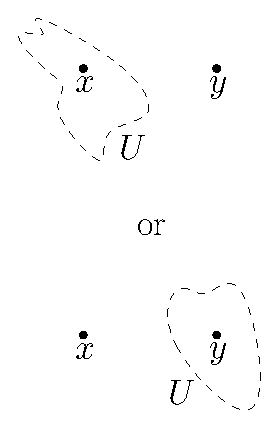
\includegraphics[height=45mm]{../img/t0.eps}
  \caption{$T_0$ property}
\end{figure}
